\documentclass[../thesis.tex]{subfiles}

\begin{document}

\chapter{Реализация} \label{chapter:implementation}

В данной главе представлено описание прототипа системы обнаружения скомпрометированных коммутаторов и результаты его экспериментального исследования.
Прототип реализует алгоритм обнаружения скомпрометированных коммутаторов, предложенный в главе \ref{chapter:algorithm}.

При реализации использовано два языка программирования: C++ \cite{stroustrup2000c++} и Python \cite{van2011python}.
На момент написания текста диссертационной работы прототип содержал $11475$ строк кода.

\section{Архитектура}

Система обнаружения скомпрометированных ПКС коммутаторов представляет собой промежуточный слой между контроллером и коммутаторами.

Эта система перехватывает OpenFlow сообщения и на их основе строит граф зависимостей правил.
Используя граф зависимостей правил, система обнаружения строит путевую развертку и устанавливает в сеть дополнительные правила маршрутизации.
При помощи статистики, полученной с этих правил, система обнаружения предсказывает значения счетчиков произвольных правил маршрутизации в сети и сравнивает их с реальными значениями, полученными из сети.

Если значения счетчиков отличаются, то система обнаружения понижает уровень доверия всех коммутаторов, влияющих на значения этого счетчика.
Такие коммутаторы находятся при помощи обхода всех путей в графе зависимостей правил, которые проходят через тестируемое правило маршрутизации.
Если уровень доверия некоторого коммутатора понижается ниже заданного порога, то система сообщает о наличии в сети скомпрометированного коммутатора.
\\

На рисунке \ref{fig:architecture} приведена схема архитектуры системы обнаружения скомпрометированных коммутаторов.
Прямоугольниками обозначены компоненты системы, стрелками --- потоки данных между компонентами.

\begin{figure}
\centering
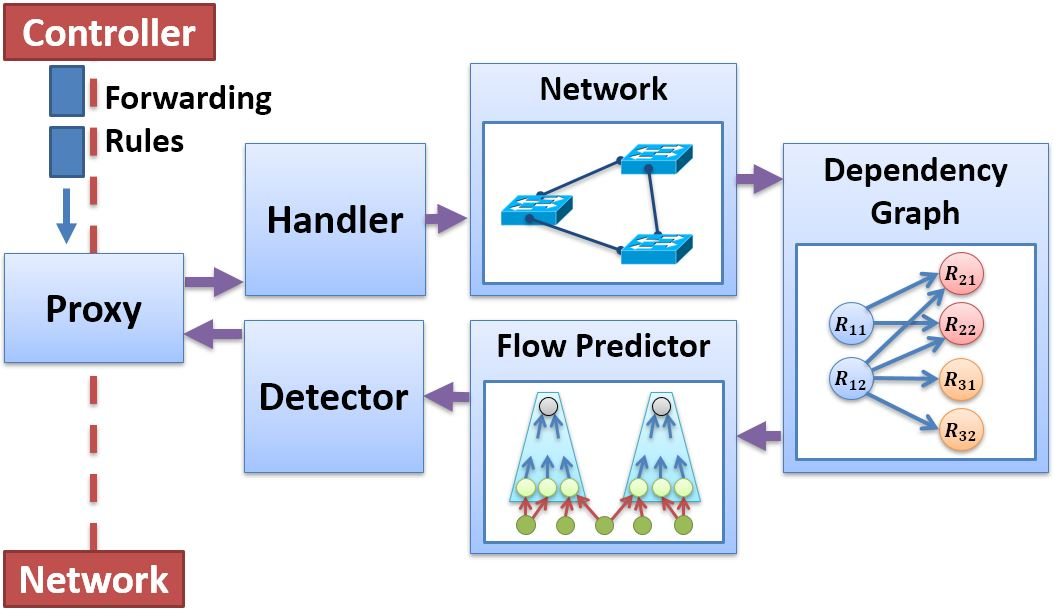
\includegraphics[width=0.8\textwidth]{figures/architecture.jpg}
\caption{Архитектура системы обнаружения} \label{fig:architecture}
\end{figure}

Модуль \textbf{\textit{Proxy}} отвечает за получение информации о топологии сети и правилах маршрутизации, установленных на коммутаторы.
Получение информации производится при помощи перехвата OpenFlow сообщений между контроллером и коммутаторами.
Перехват сообщений необходим для построения графа зависимостей правил, описывающего состояние сети.

Модуль \textbf{\textit{Handler}} отвечает за обработку OpenFlow сообщений, перехваченных модулем \textit{Proxy}.
Этот модуль также преобразует OpenFlow сообщения во внутреннее представление программы, а именно представление полей \textit{match} в виде \textit{wildcard} масок модели \textit{Header Space}.
\\

Модуль \textbf{\textit{Network}} представляет собой базу данных, хранящую информацию о текущем состоянии сети.
Под этой информацией понимается: список коммутаторов с их свойствами, список портов и таблиц маршрутизации, топология сети и правила маршрутизации установленные на коммутаторах.

Модуль \textbf{\textit{Dependency Graph}} строит граф зависимостей правил на основе событий, изменяющих состояние сети.
Этот модуль также предоставляет интерфейс к графу зависимостей правил для других модулей системы.

Модуль \textbf{\textit{Flow Predictor}} отвечает за предсказание значений счетчиков правил маршрутизации.
Модуль строит путевую развертку на основе графа зависимостей правил и использует ее для создания и установки в сеть дополнительных правил маршрутизации.
Модуль также запрашивает статистику с этих правил маршрутизации для предсказания значений счетчиков произвольных правил маршрутизации.

Модуль \textbf{\textit{Detector}} отвечает за обнаружение скомпрометированных коммутаторов, основываясь на данных, предоставляемых модулями \textit{Dependency Graph} и \textit{Flow Predictor}.

\pagebreak
\section{Экспериментальная проверка предложенного решения}

В этой главе описаны результаты экспериментальной проверки предложенного решения для обнаружения скомпрометированных коммутаторов.

\subsection{Методика испытаний}

Экспериментальное исследование нацелено на определение следующих свойств предложенного решения:
\begin{enumerate}
\item Погрешность предсказания значений счетчиков;
\item Время работы алгоритма;
\item Ошибки первого и второго рода при обнаружении.
\end{enumerate}

Под ошибками первого рода понимаются ситуации, когда легитимный коммутатор был классифицирован как скомпрометированный.
Под ошибками второго рода понимаются ситуации, когда скомпрометированный коммутатор был классифицирован системой обнаружения как легитимный.

\subsubsection{Погрешность предсказания значений счетчиков}

Под погрешностью предсказания счетчиков маршрутизации понимается величина, равная разности реального знаечния счетчика и предсказанного.

Погрешность предсказания влияет на ошибки первого рода при обнаружении скомпрометированных коммутаторов, так как наличие отклонения предсказанных значений счетчиков от реальных влияет на уровни доверия коммутаторов.

На погрешность предсказания значений счетчиков влияют следующие факторы:
\begin{enumerate}
\item Задержки обработки трафика;
\item Объемы потоков данных.
\end{enumerate}

\textit{Задержки обработки трафика}

Под задержками обработки трафика понимается сумма следующих величин:
\begin{enumerate}
\item Задержек распространения --- времени прохождения сигнала по каналам данных;
\item Задержек пакетизации --- времени, за которое биты пакета с первого до последнего переданы в канал;
\item Задержек в буфере коммутатора --- времени, которое пакеты проводят в ожидании обработки коммутатором.
\end{enumerate}

Задержки влияют на погрешность предсказания, потому что предсказание счетчиков основывается на запросах статистики с дополнительных правил маршрутизации.
Во время запроса статистики из сети, часть пакетов, обработанных дополнительными правилами маршрутизации, может не успеть дойти по сети до анализируемого правила.
Разница в этих пакетах будет отражаться в разнице между предсказанным и реальным значением счетчика анализируемого правила.

\textit{Объемы потоков данных}

Объемы потоков данных, проходящих через коммутаторы в сети, влияют на погрешность предсказания значений счетчиков в совокупности с задержками обработки пакетов.
Чем больше объем трафика в сети, тем больше пакетов не успеет дойти до анализируемого правила, и тем больше будет различие между реальными и предсказанными значениями счетчика анализируемого правила.

\subsubsection{Время работы алгоритма}

Система обнаружения перехватывает и ставит в очередь OpenFlow сообщения от контроллера, которые описывают установку правил маршрутизации.
Очередь необходима для того, чтобы создавать дополнительные правила маршрутизации и устанавливать их одновременно с оригинальными правилами, созданными контроллером.

Наличие этой очереди замедляет реакцию контроллера на события в сети, потому что правила маршрутизации устанавливаются с задержкой.
Эта задержка зависит от времени работы алгоритма, а именно времени построения графа зависимостей правил и путевой развертки, которое в свою очередь зависит от размера сети и количества правил маршрутизации, установленных в сеть.

Таким образом, необходимо оценить время работы алгоритма в зависимости от:
\begin{enumerate}
\item Размера сети;
\item Количества правил маршрутизации.
\end{enumerate}

\subsubsection{Ошибки первого и второго рода при обнаружении}

Основная задача алгоритма --- обнаружение скомпрометированных коммутаторов.
Поэтому необходимо, во-первых, экспериментально показать корректность работы алгоритма, и во-вторых, оценить ошибки первого и второго рода.

Была исследована зависимость ошибок первого и второго рода от следующих факторов:
\begin{enumerate}
\item Размера сети;
\item Количества правил;
\item Объемов потоков данных;
\item Типа атаки;
\item Длительности атаки;
\item Количества скомпрометированных коммутаторов.
\end{enumerate}

Необходимо отметить, что величина ошибок первого и второго рода зависит от всех факторов, влияющих на точность предсказания счетчиков.

\subsubsection{Тестовый стенд}

Для реализации экспериментального исследования был разработан тестовый стенд на основе библиотеки \textit{Mininet} \cite{lantz2010network}.
Эта библиотека позволяет создавать виртуальные сети из программных коммутаторов и также создавать искусственные задержки в сети.
В качестве коммутаторов использовались программные коммутаторы \textit{Open vSwitch} \cite{pfaff2015design}.

В качестве тестовых топологий сети использовались топологии из библиотеки \textit{TopologyZoo} \cite{knight2011internet}.
Эта библиотека содержит 522 топологии, описывающих реальные топологии сетей телеком операторов.
Также для экспериментов использовались линейные топологии и топологии типа \textit{Tree} и \textit{FatTree} \cite{al2008scalable}, которые часто используются в центрах обработки данных \cite{saino2013toolchain}.
Размеры топологий варьировались от 5 до 300 коммутаторов.
В качестве тестового ПКС контроллера использовался контроллер RunOS \cite{shalimov2015runos}.

Виртуальная сеть с программными коммутаторами была запущена на сервере со следующими характеристиками:
\begin{enumerate}
\item ЦПУ (Центральное процессорное устройство) --- Intel\textsuperscript{\textregistered} Xeon\textsuperscript{\textregistered} E5-2620 v4, 32 ядра по 2.10GHz;
\item ОЗУ (Оперативное запоминающее устройство) --- 32 Gb DDR3 1333 MHz;
\item Сетевой интерфейс --- 1 Gb Ethernet.
\end{enumerate}

Контроллер был запущен на виртуальной машине, находящейся на отдельном сервере со следующими характеристиками:
\begin{enumerate}
\item ЦПУ (Центральное процессорное устройство) --- Intel\textsuperscript{\textregistered} Core\textsuperscript{\textregistered} i7 9xx (Nehalem Class Core i7), 2 ядра по 2.4 GHz;
\item ОЗУ (Оперативное запоминающее устройство) --- 2 Gb DDR3 1333 MHz;
\item Сетевой интерфейс --- 1 Gb Ethernet.
\end{enumerate}

Среднее время работы алгоритма определялось следующим образом.
Эксперименты проводились по 10 раз на каждой топологии.
После каждого запуска измерялась задержка установки правил маршрутизации.
Все времена суммировались и усреднялись по числу запусков.
Полученная величина бралась за среднее время выполнения программы.

Для определения погрешности предсказания значений счетчиков в сети создавалась искуственная задержка и измерялась разность в значениях предсказанных и реальных счетчиков правил маршрутизации.

Для проверки корректности работы алгоритма в сеть случайно добавлялись правила сбрасывающие, дублирующие и некорректно маршрутизирующие трафик.
Далее проверялось, что алгоритм корректно обнаружил скомпрометированные коммутаторы, и вычислялись величины ошибки первого и второго рода.

\subsection{Результаты испытаний}

\subsubsection{Погрешность предсказания значений счетчиков}

\begin{figure}
\centering
\captionsetup{justification=centering,margin=2cm}
\begin{subfigure}[b]{0.49\textwidth}
  \centering
  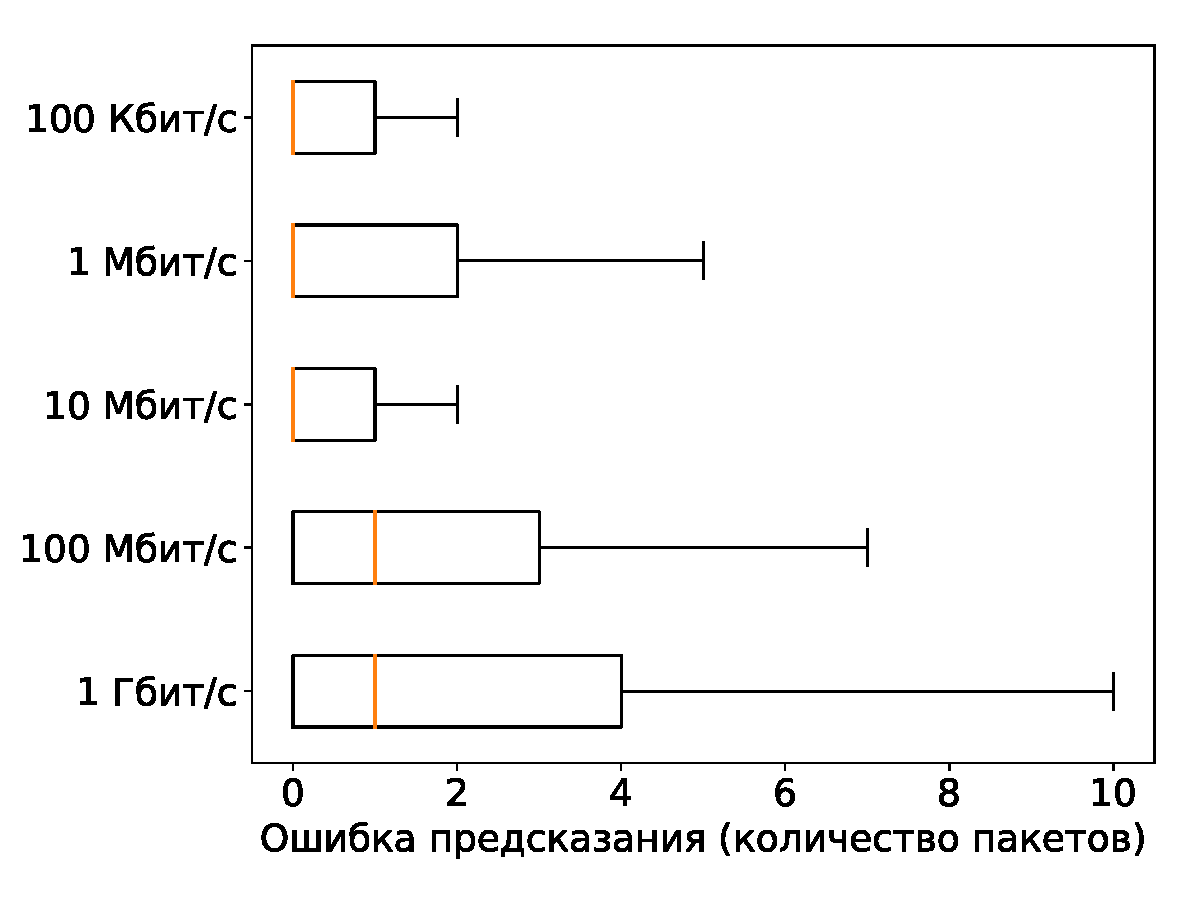
\includegraphics[width=1.0\textwidth]{figures/experiments/packet_error_5.pdf}
  \caption{Задержка < 1 мс} \label{fig:prediction_error_1}
\end{subfigure}
\begin{subfigure}[b]{0.49\textwidth}
  \centering
  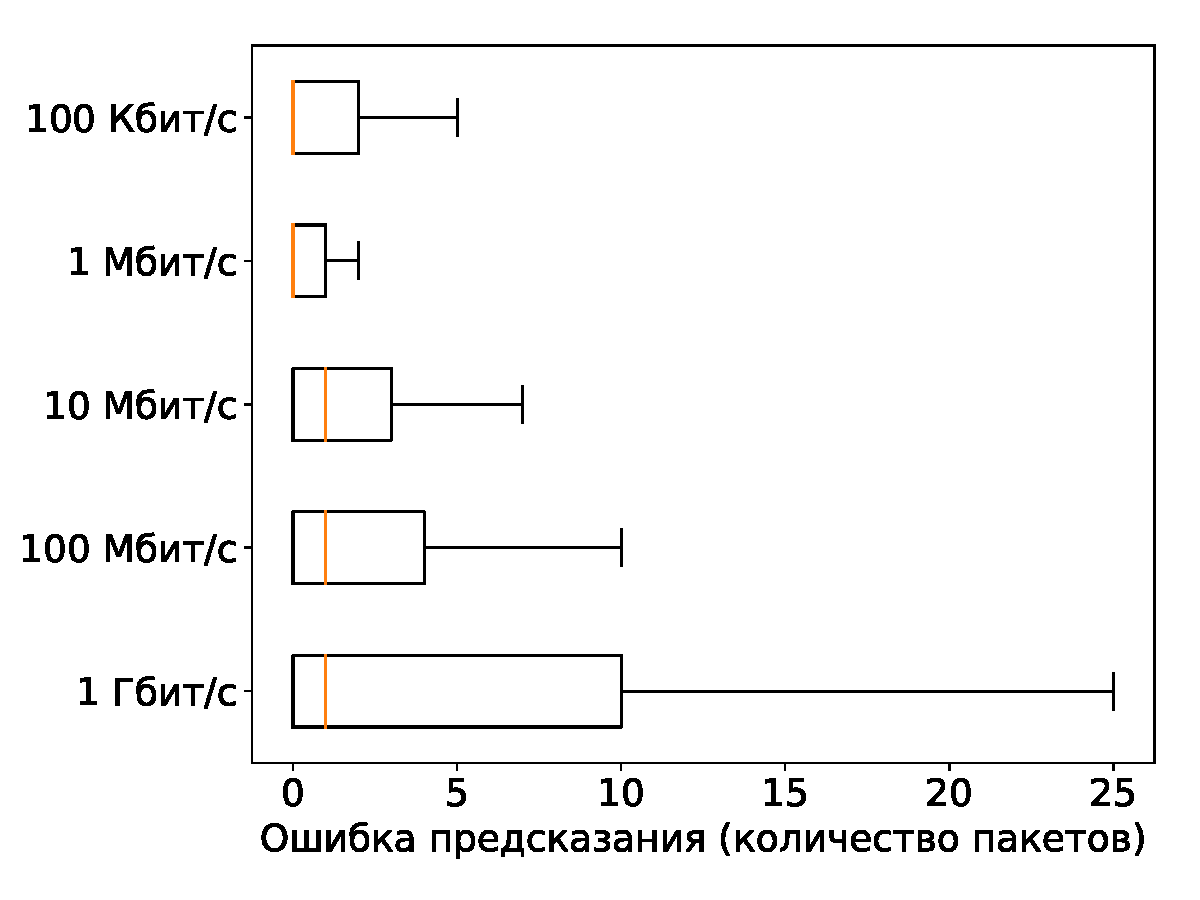
\includegraphics[width=1.0\textwidth]{figures/experiments/packet_error_10.pdf}
  \caption{Задержка 5 мс} \label{fig:prediction_error_5}
\end{subfigure}
\begin{subfigure}[b]{0.49\textwidth}
  \centering
  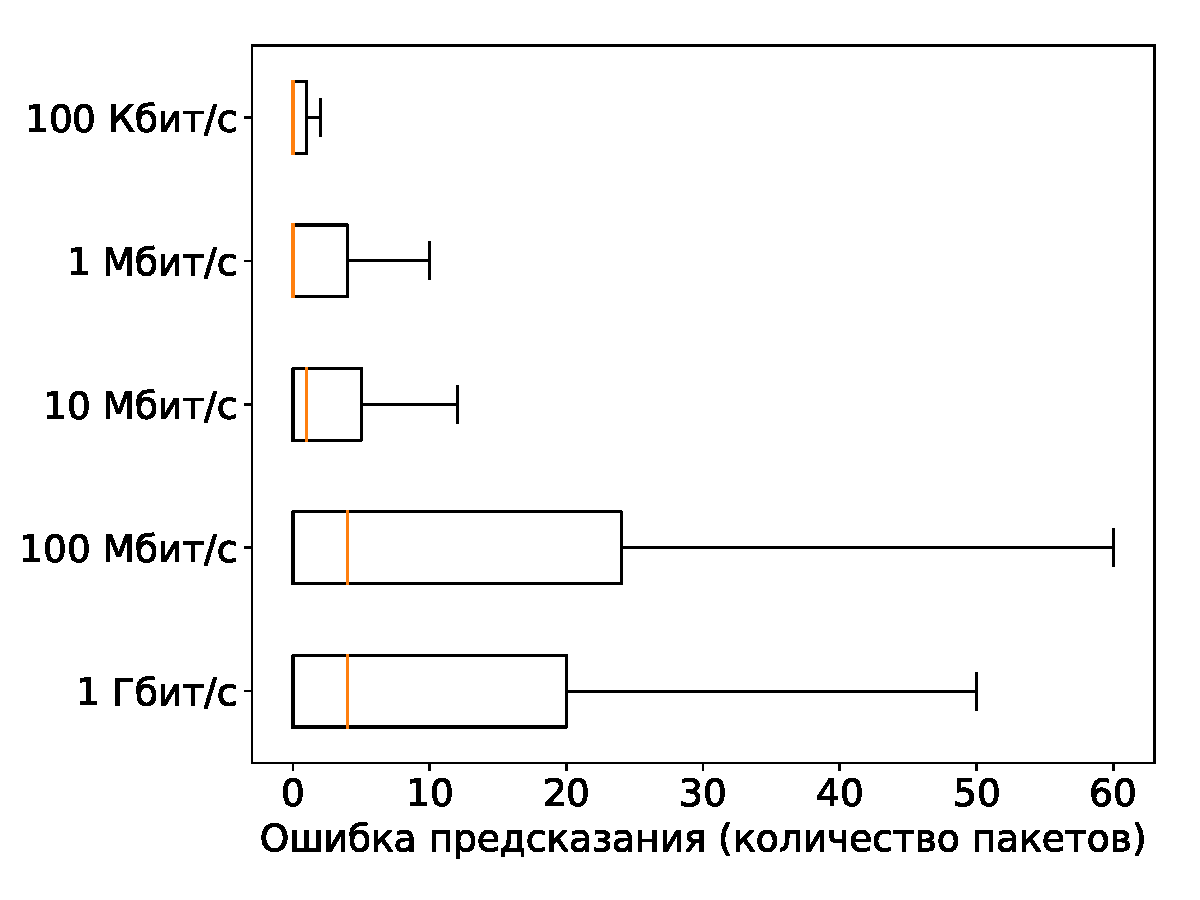
\includegraphics[width=1.0\textwidth]{figures/experiments/packet_error_50.pdf}
  \caption{Задержка 10 мс} \label{fig:prediction_error_10}
\end{subfigure}
\begin{subfigure}[b]{0.49\textwidth}
  \centering
  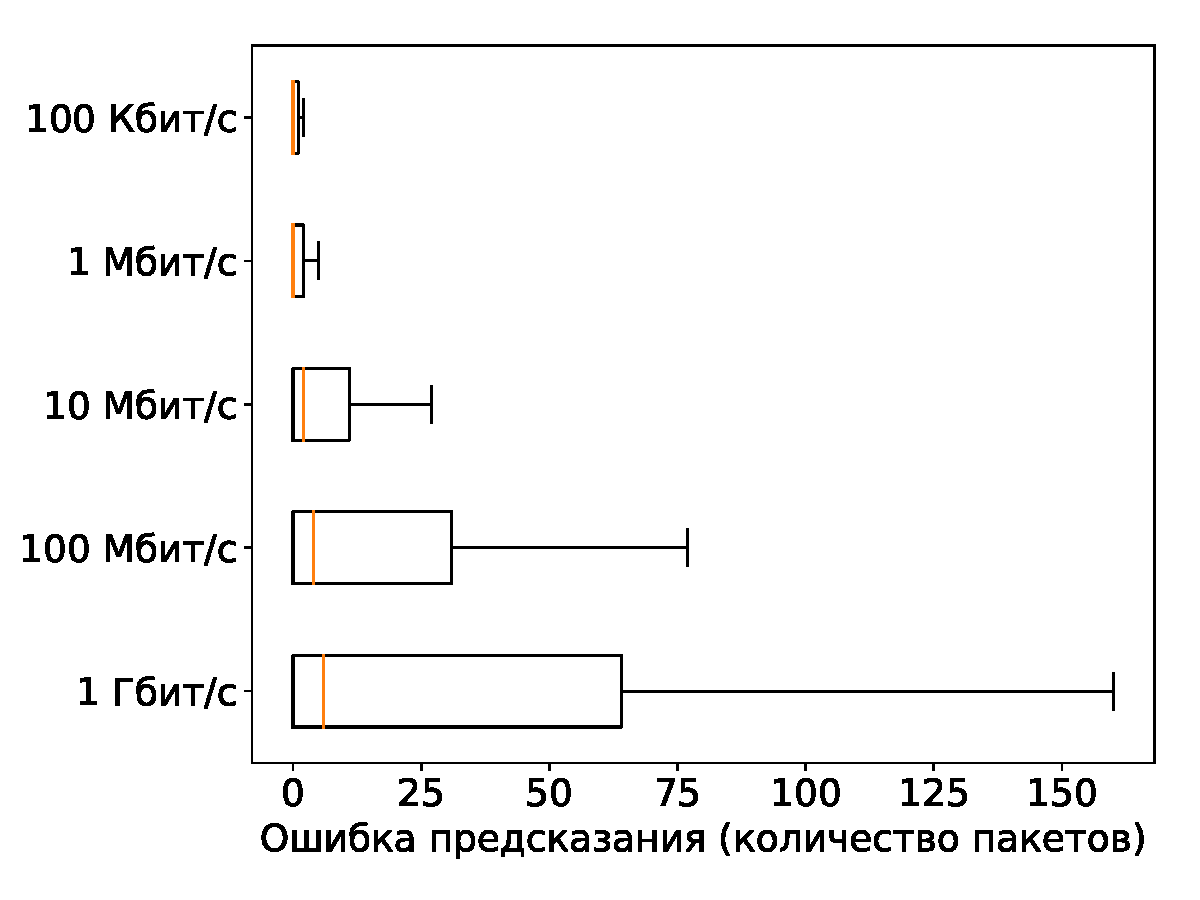
\includegraphics[width=1.0\textwidth]{figures/experiments/packet_error_100.pdf}
  \caption{Задержка 50 мс} \label{fig:prediction_error_50}
\end{subfigure}
\begin{subfigure}[b]{0.49\textwidth}
  \centering
  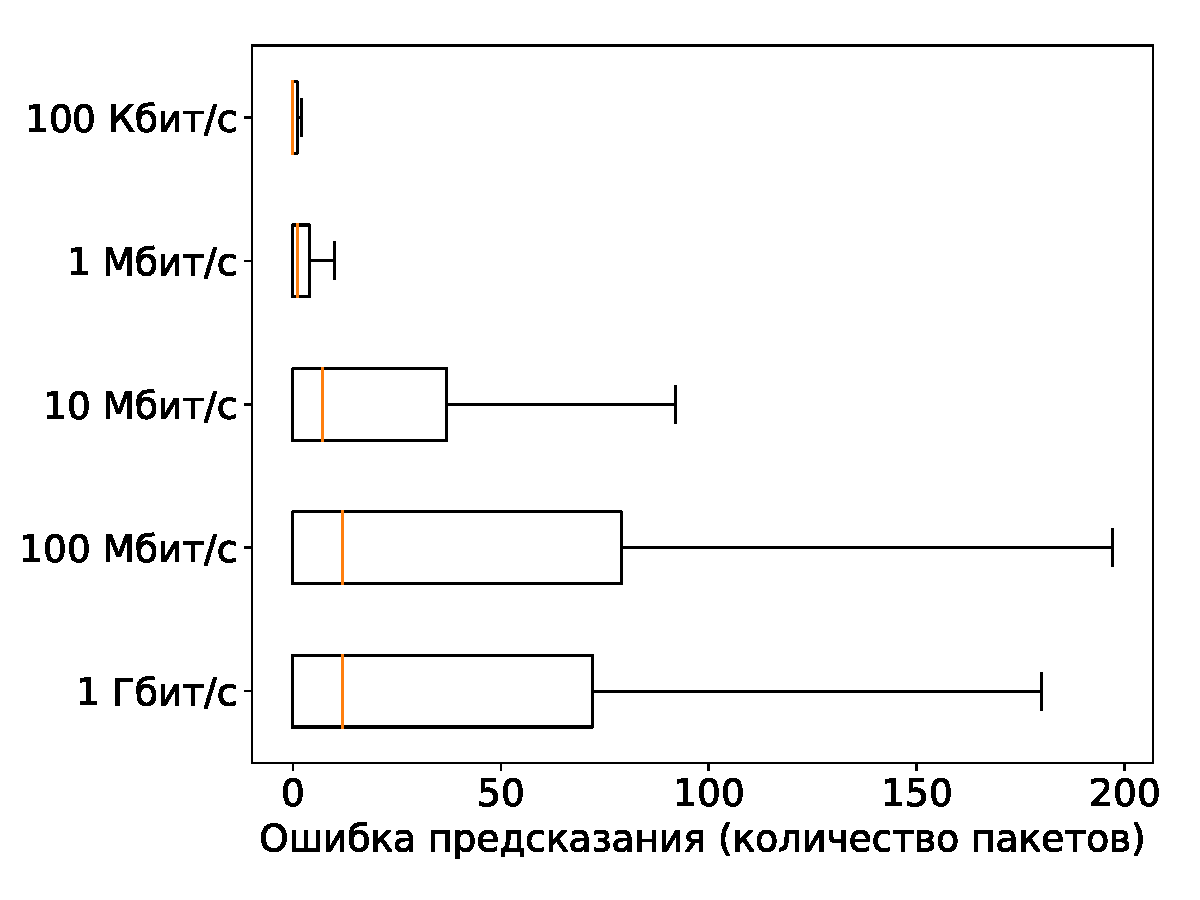
\includegraphics[width=1.0\textwidth]{figures/experiments/packet_error_300.pdf}
  \caption{Задержка 100 мс} \label{fig:prediction_error_100}
\end{subfigure}
\begin{subfigure}[b]{0.49\textwidth}
  \centering
  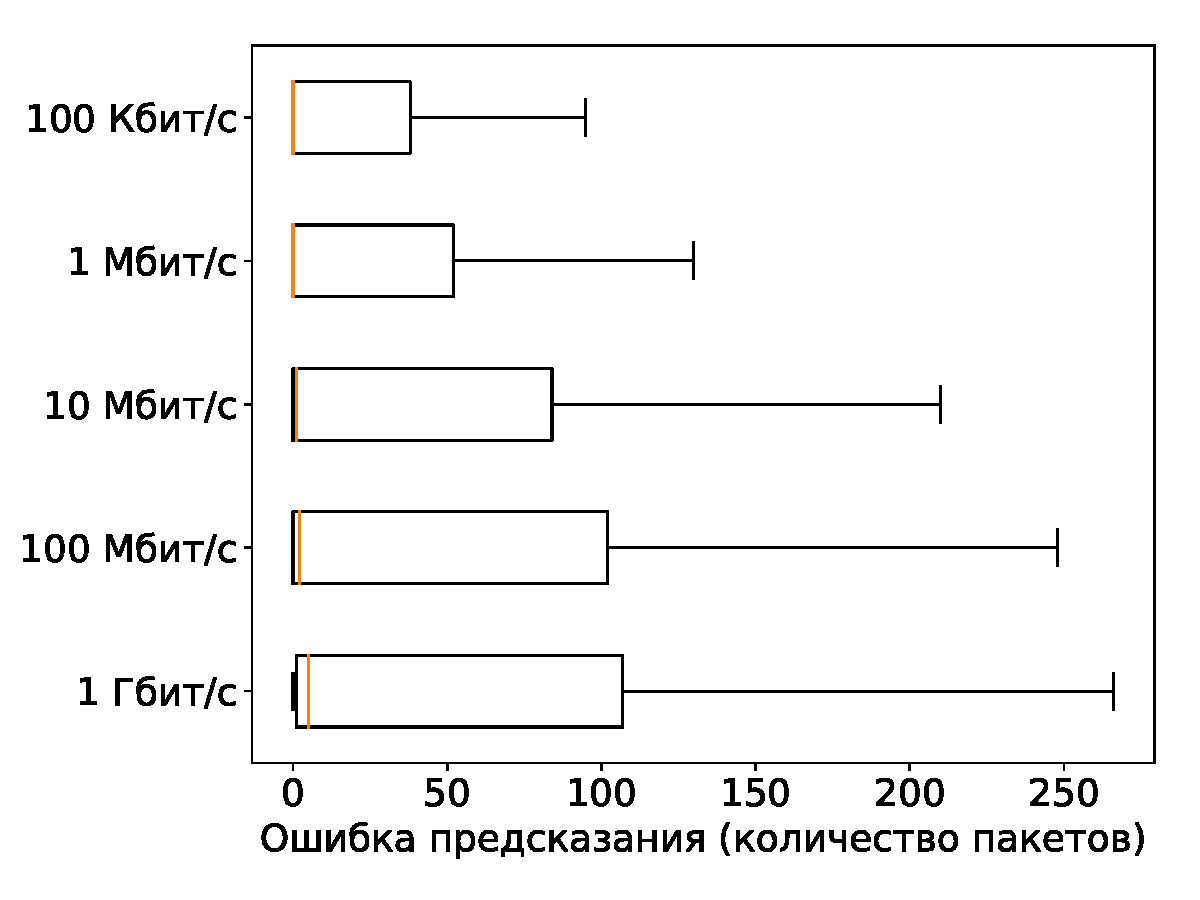
\includegraphics[width=1.0\textwidth]{figures/experiments/packet_error.pdf}
  \caption{Задержка 300 мс} \label{fig:prediction_error_300}
\end{subfigure}
\caption{Зависимость ошибки предсказания счетчика от объема потоков данных} \label{fig:prediction_error}
\end{figure}

На рисунке \ref{fig:prediction_error} показана зависимость погрешности предсказания счетчика (разница между реальными и предсказанными значениями счетчиков) от объема потоков данных.

На рисунке также показана зависимость погрешности от задержек в сети.
Под задержкой понимается средняя сквозная (\textit{end-to-end}) задержка для всех пар подключенных клиентов.

График представляет собой \textit{box-plot}, описываемый следующим образом:
\begin{enumerate}
\item Оранжевой линией показана медиана значений погрешности;
\item Прямоугольником показаны первая и третья квартили, отделяющие 25\% и 75\% значений погрешности соответственно;
\item Штрихами показан 95\%-ый доверительный интервал.
\end{enumerate}
Под 95\%-ым доверительный интервал показывает, что 95\%-ов значений выборки принадлежат этому интервалу.

Согласно результатам тестирования погрешность практически одинакова для объемов потоков данных 100 Кбит/с до 10 Мбит/с и начинает возрастать для потоков объемом более 100 Мбит/с.
Также при сквозной задержке в 300 мс погрешность начинает возрастать до 100 пакетов даже для потоков объемом 100 Кбит/с.
Это объясняется тем, что из-за больших значений задержки, большое количество пакетов не успевает пройти от дополнительных правил на границе сети до анализируемого правила.

Тестирование также показало, что максимальный порог легитимных отклонений, превышение которого может свидетельствовать о наличии в сети атаки, равен 270 пакетам.

\subsubsection{Время работы алгоритма}

\begin{figure}
\centering
\captionsetup{justification=centering,margin=2cm}
\begin{subfigure}[b]{0.49\textwidth}
  \centering
  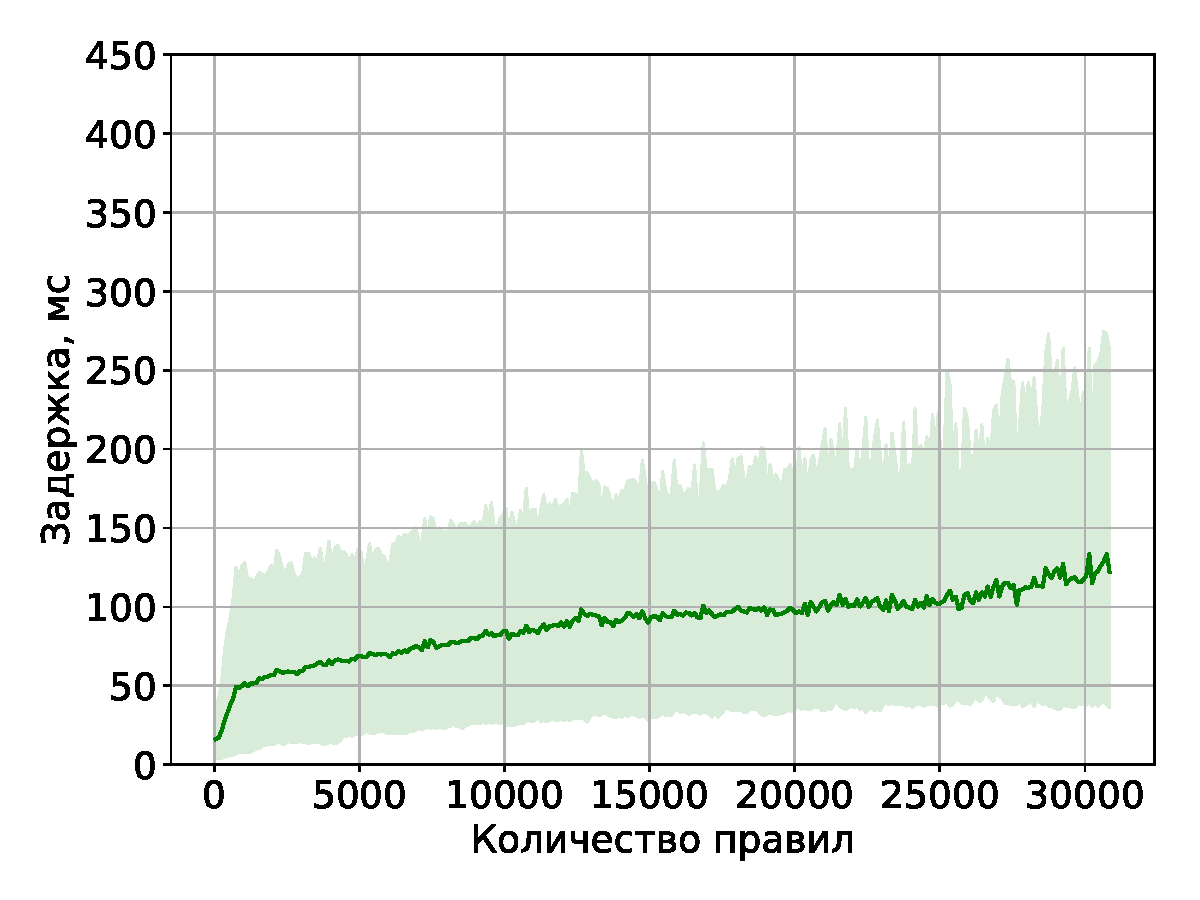
\includegraphics[width=1.0\textwidth]{figures/experiments/delay_by_rules_0_100.pdf}
  \caption{От 5 до 100 коммутаторов} \label{fig:delay_by_rules_5_100}
\end{subfigure}
\begin{subfigure}[b]{0.49\textwidth}
  \centering
  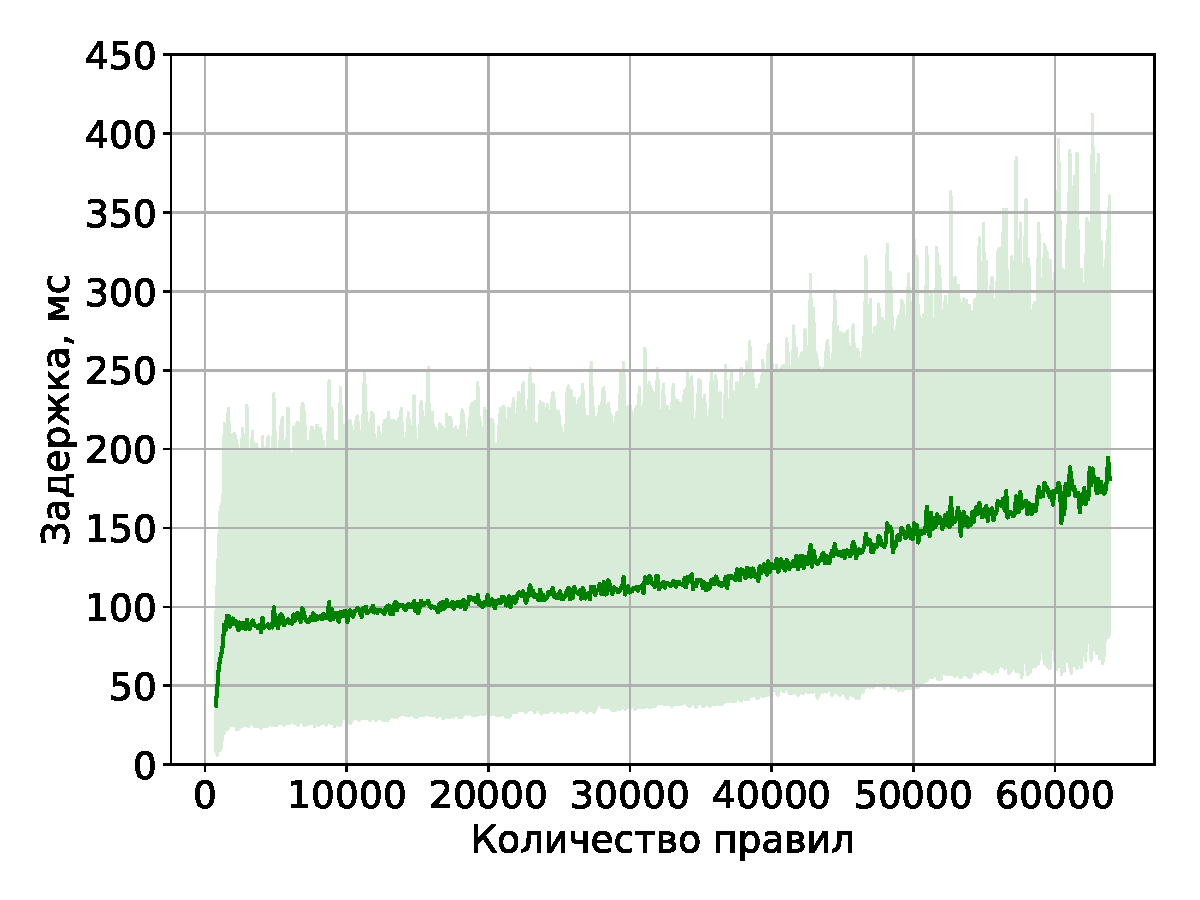
\includegraphics[width=1.0\textwidth]{figures/experiments/delay_by_rules_100_200.pdf}
  \caption{От 100 до 200 коммутаторов} \label{fig:delay_by_rules_100_200}
\end{subfigure}
\begin{subfigure}[b]{0.49\textwidth}
  \centering
  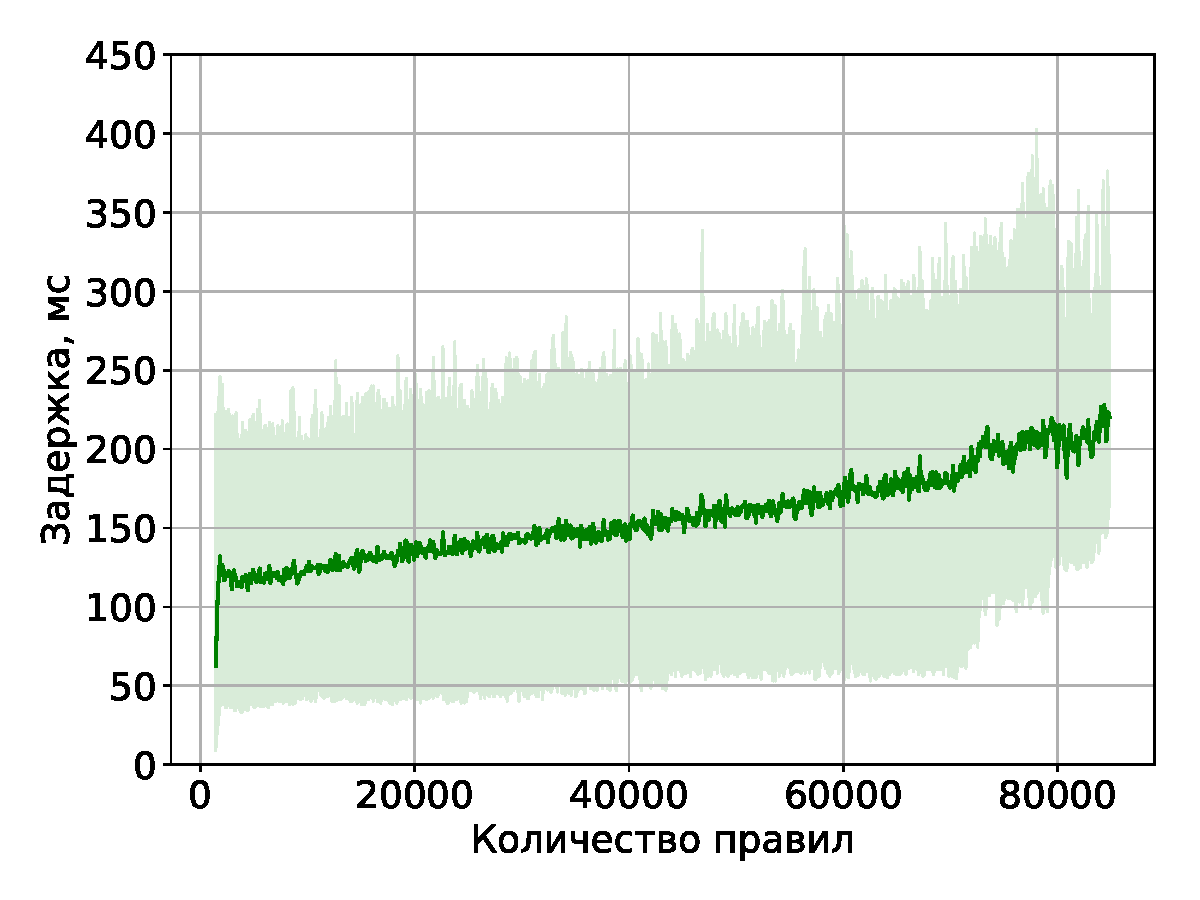
\includegraphics[width=1.0\textwidth]{figures/experiments/delay_by_rules_200_250.pdf}
  \caption{От 200 до 250 коммутаторов} \label{fig:delay_by_rules_200_250}
\end{subfigure}
\begin{subfigure}[b]{0.49\textwidth}
  \centering
  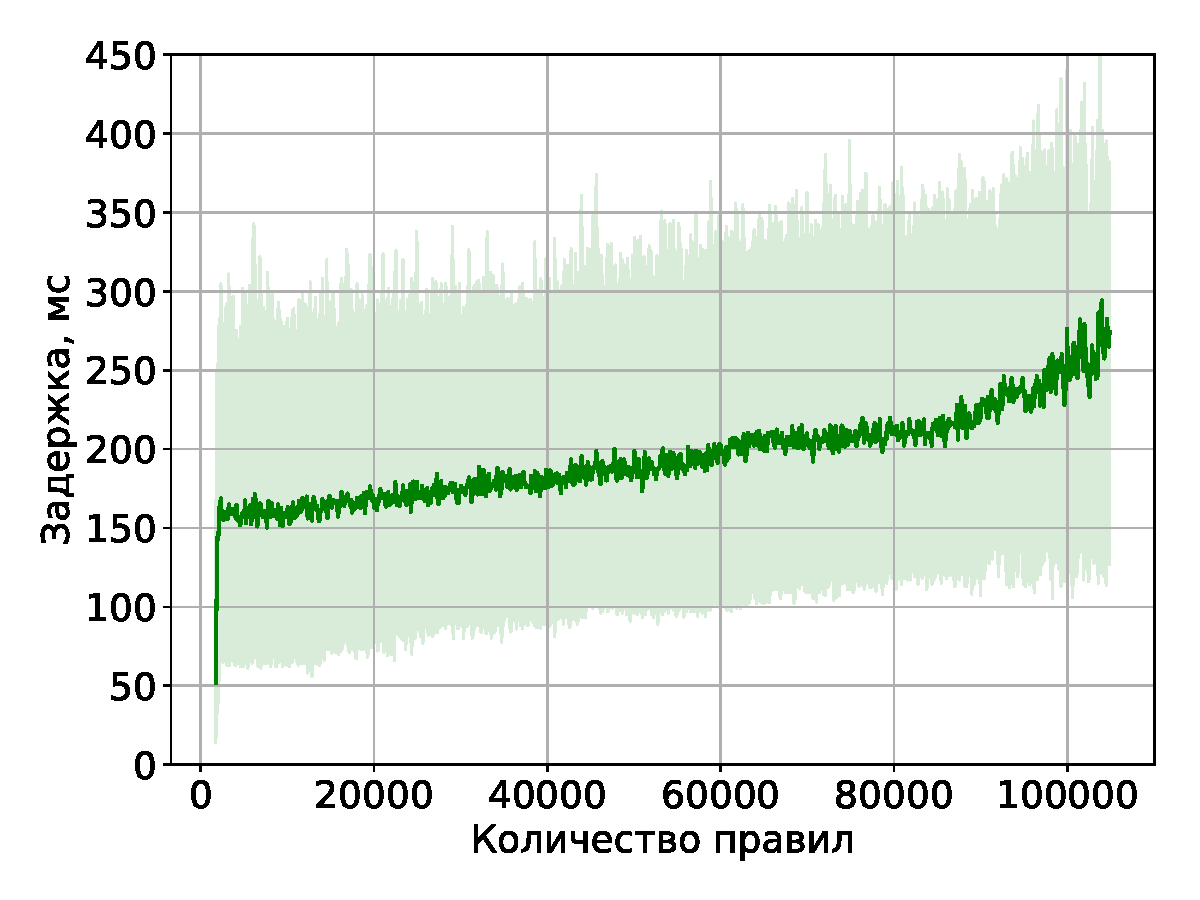
\includegraphics[width=1.0\textwidth]{figures/experiments/delay_by_rules_250_300.pdf}
  \caption{От 250 до 300 коммутаторов} \label{fig:delay_by_rules_250_300}
\end{subfigure}
\caption{Зависимость задержки от количества коммутаторов и правил в сети и размера топологии} \label{fig:delay_by_rules}
\end{figure}

\begin{figure}
\centering
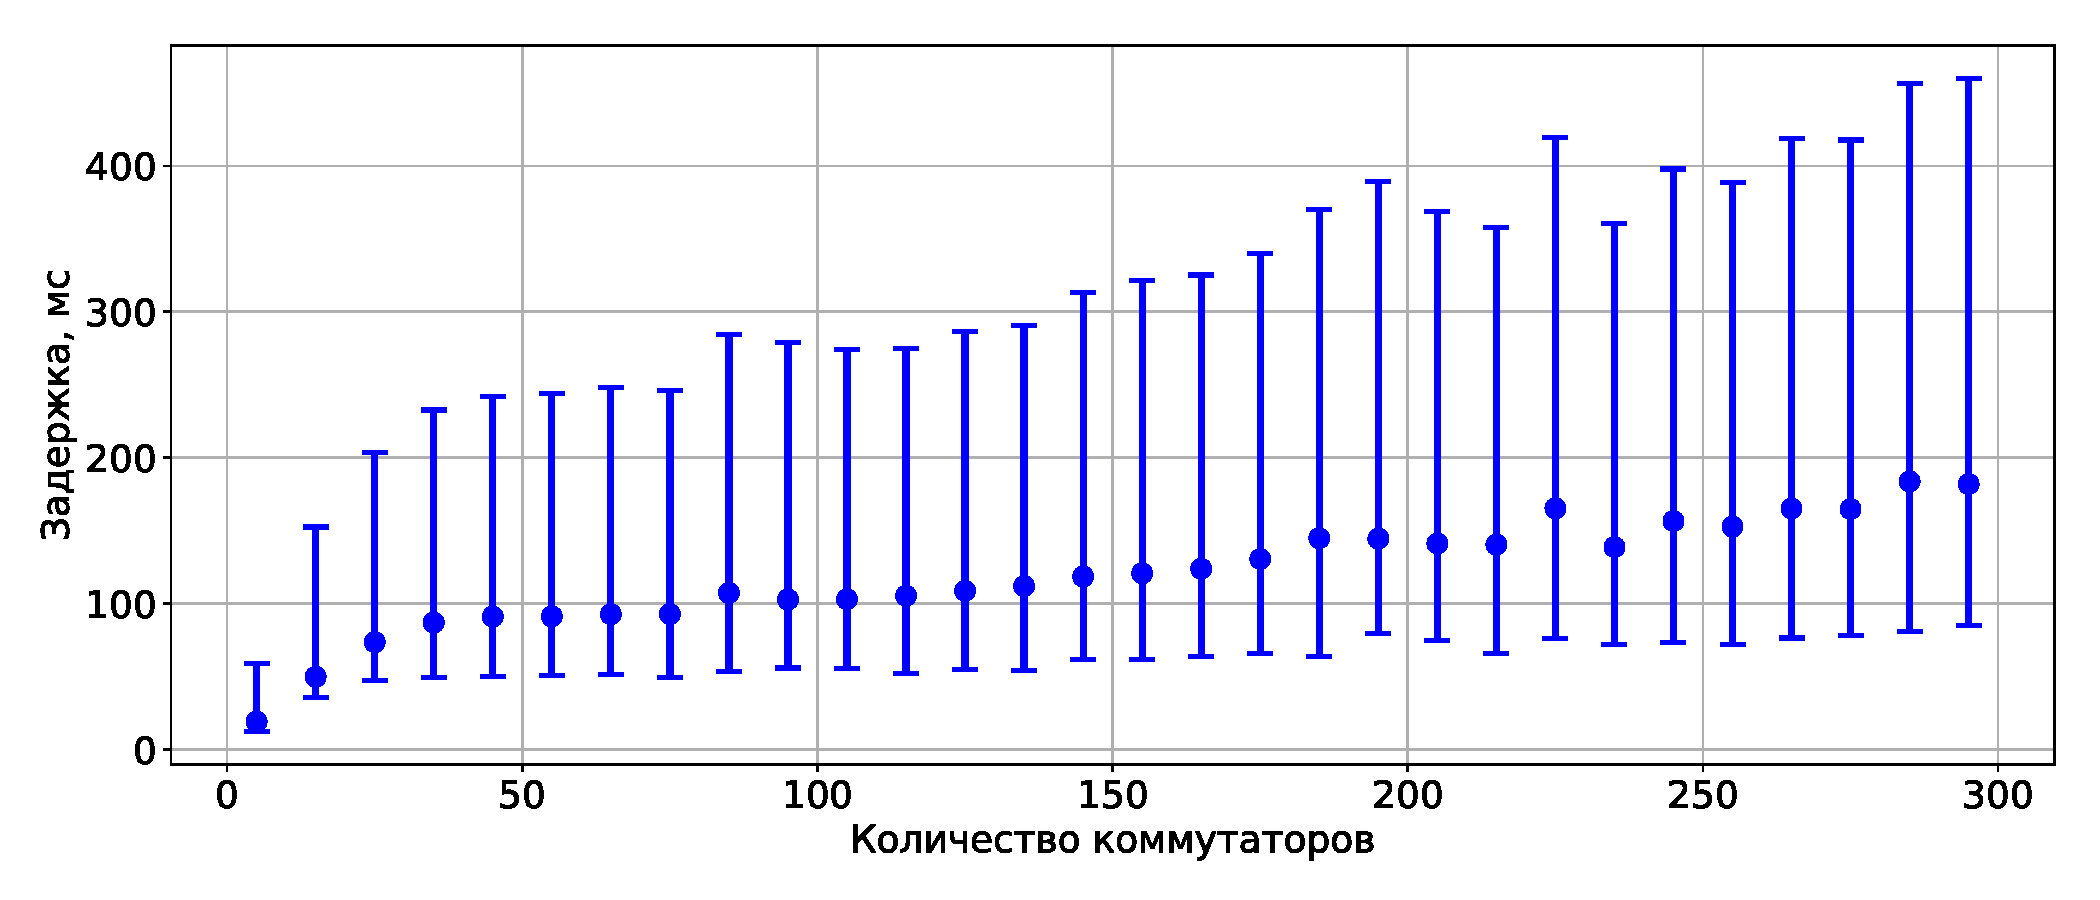
\includegraphics[width=0.92\textwidth]{figures/experiments/delay_by_switches.pdf}
\caption{Зависимость задержки от количества коммутаторов в сети} \label{fig:delay_by_switches}
\end{figure}

На рисунке \ref{fig:delay_by_rules} показана зависимость задержки от количества правил в сети и размера топологии.
Линией на графиках показано среднее значение времени работы алгоритма а закрашенными областями --- 95\%-ый доверительный интервал.

На рисунке \ref{fig:delay_by_switches} показана зависимость задержки от количества коммутаторов в сети усредненная по различным топологиям с одинаковым количеством коммутаторов.
Точкой на графике показано среднее значение а интервалами --- 95\%-е доверительные интервалы.

Результаты экспериментов показывают, что время работы алгоритма, увеличивается с увеличением количества правил, установленных в сеть.
Задержки могут быть ограничены сверху 420 миллисекундами для больших топологий (300 коммутаторов) с большим количеством правил (100.000).
Также стоит отметить, что время работы алгоритма линейно возрастает с увеличением количества правил маршрутизации.

\subsubsection{Точность обнаружения скомпрометированных коммутаторов}

{
\newcolumntype{Y}{>{\centering\arraybackslash}X}

\begin{table}[htbp]
\centering
\begin{tabularx}{\textwidth}{|c|Y|Y|}
  \hline
  \textbf{Тип атаки} & \textbf{FP} & \textbf{FN} \\ \hline
  Отсутствие атаки & 0.002 & n/a \\ \hline
  Некорректная маршрутизация & 0.008 & 0.019 \\ \hline
  Дублирование трафика & 0.023 & 0.049 \\ \hline
  Сброс трафика & 0.037 & 0.066 \\ \hline
\end{tabularx}
\caption{Ошибки первого (FP) и второго рода (FN) при обнаружении} \label{table:detection}
\end{table}
}

\begin{figure}
\centering
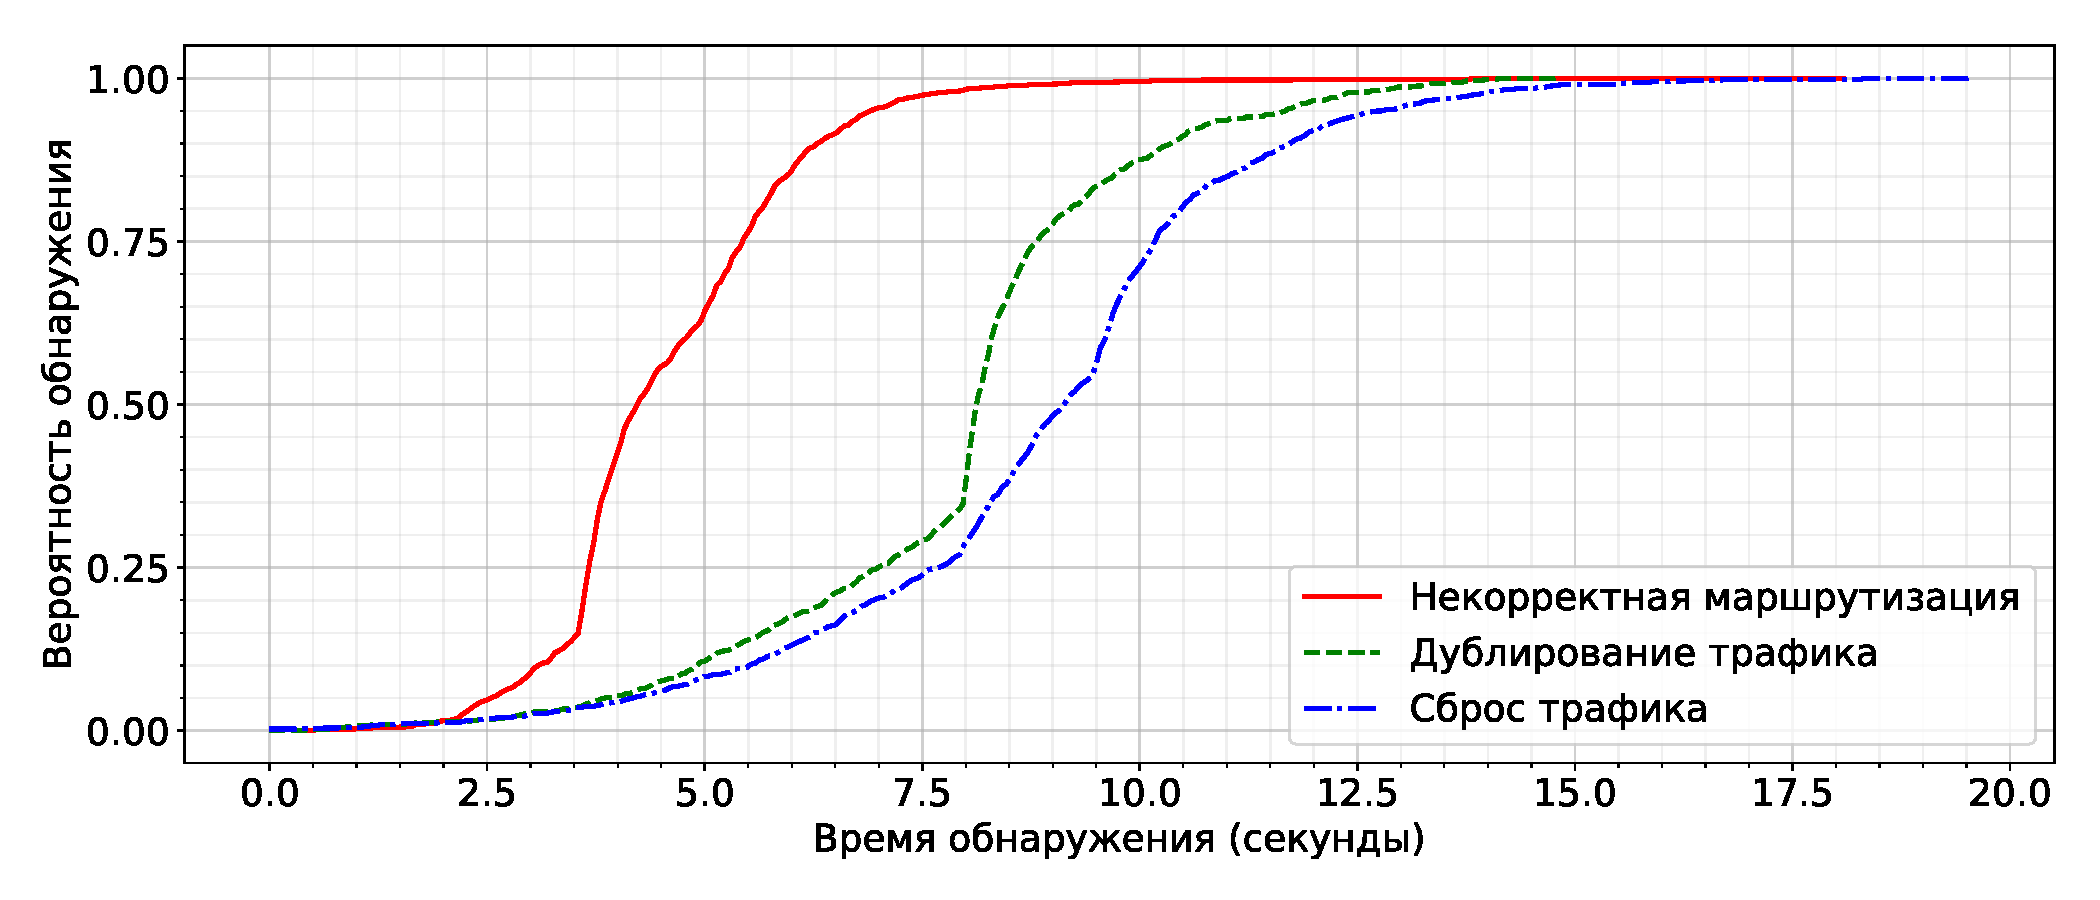
\includegraphics[width=0.92\textwidth]{figures/experiments/detection.pdf}
\caption{Функция распределения вероятности обнаружения} \label{fig:detection_cdf}
\end{figure}

В таблице \ref{table:detection} показаны ошибки первого и второго рода при обнаружении скомпрометированных коммутаторов.
Ошибки второго рода при отсутствии атаки не имеют смысла (\textbf{n/a}), так как ошибка второго рода описывает ситуации, когда скомпрометированный коммутатор был классифицирован как легитимный.
Результаты экспериментов показывают, что ошибки первого рода происходят в 3.7\% случаев, а ошибки второго рода --- в 6.6\% случаев.

Меньшее количество ошибок при некорректной маршрутизации объясняется тем, что эта атака затрагивает как минимум 2 доменных пути --- новый маршрут трафика и старый маршрут, по которому должен был идти трафик, таким образом, повышая вероятность нахождения некорректного значения счетчика.

Также необходимо отметить, что более 90\% от всех ошибок возникало на больших топологиях --- более 240 коммутаторов.

На рисунке \ref{fig:detection_cdf} показано время обнаружения скомпрометированных коммутаторов в зависимости от типа атаки и объемов потоков данных.
Графики представляют собой функции распределения, где случайной величиной является время обнаружения скомпрометированного коммутатора.
Необходимо отметить, что в построении графика участвовали только данные, на которых скомпрометированный коммутатор был обнаружен корректно.
Интервал проверки в экспериментах был выбран равным 10 мс --- так как меньший интервал может привести к перегрузкам управляющего канала \cite{chowdhury2014payless}.

Результаты экспериментов показывают, что с вероятностью 90\% некорректная маршрутизация будет обнаружена менее чем за 6.5 секунд после начала атаки, дублирование трафика менее чем за 10.5 секунд и сброс трафика менее чем за 11.9 секунд.

\section{Выводы}

В главе описана реализация алгоритма обнаружения скомпрометированных коммутаторов в ПКС и описаны результаты экспериментального исследования.

Эксперименты на топологиях размером до 300 коммутаторов и интенсивности потоков до 1 Гбит/с показывают, что предложенный алгоритм способен обнаружить скомпрометированный коммутатор менее, чем через 15 секунд после начала атаки, при этом ошибки первого и второго рода составляют 3.7\% и 6.6\% соответственно.
Также негативное влияние на сеть, представляемое задержками реакции контроллера на изменение состояния сети, не превышает 420 мс.

\end{document}